\documentclass[12pt]{scrartcl} %Dokumentklasse, bestimmt Teile des Layouts
\usepackage[utf8]{inputenc} %Ermöglicht Unicode, absolut notwendig
\usepackage[ngerman]{babel} %Ermöglicht deutsche Sonderzeichen, z. B. Umlaute
\usepackage[T1]{fontenc} %Ermöglicht Unicode, absolut notwendig
\usepackage{amsmath} %Wichtige Mathe-Möglichkeiten
\usepackage{amssymb} %Wichtige Mathe-Möglichkeiten
\usepackage{epstopdf} %Um .eps-Bilder in Latex verwenden zu können
\usepackage[onehalfspacing]{setspace} %Bestimmt den Zeilenabstand, hier 1,5
\usepackage{graphicx} %Bessere Bilder
\usepackage{array} %Bessere Formatierung / Umgebung für mehrzeilige Formeln
\usepackage{upgreek} %Für nicht kursive griechische Buchstaben, z. B. \upmu statt \mu
\usepackage{float} %Großes H zum fixieren von Abbildungen/Tabellen
%\usepackage{csquotes}% Anführungszeichen etc.
\usepackage{mhchem}% für Chemische Formeln und Reaktionsgleichungen
\usepackage{tikz} %Vektorgrafziken im LaTeX-eigenen Format, z. B. zum Export aus QtiPlot
\usepackage{graphicx}
\usepackage[font=small]{caption} %Bestimmt die Schriftgröße von Tabellenüberschriften und Bildunterschriften, optional
\usepackage[backend=biber, style=chem-angew]{biblatex} %Literaturverzeichnis
\usepackage{tabularx, booktabs, multirow} %Für bessere Tabellen und einfachen Excel to Latex import
\usepackage[
  left=3cm,
  right=2cm
]{geometry}
\usepackage{pgfplots}
\newcommand{\celsius}{^{\circ}\mathrm{C}} %Ermöglicht es, \celsius für die Einheit °C zu verwenden
\geometry{bottom=100pt} \geometry{top=100pt} %Definiert den oberen und unteren Rand, optional
\parindent0pt %Kein Einzug am Anfang von Absätzen
\sloppy %Besserer Blocksatz
\renewcaptionname{ngerman}{\figurename}{Abb.} %Umbenennung Abbildungen, optional
\renewcaptionname{ngerman}{\tablename}{Tab.} %Umbenennung Tabellen, optional
\begin{document}
\begin{titlepage}
\begin{center}
\vspace*{2cm}
\begin{LARGE}
\vspace*{1cm}
\textbf{\textsf{Quantitative Analyse - Aufgabe 4\\}}
\end{LARGE}
\vspace*{1cm}
\textbf{\textsf{Praktikum zur analystischen Chemie}}\\
\vspace*{1.5cm}
\begin{table}[H]
\sffamily
\hspace*{3cm}\begin{tabular}{>{\bfseries}l>{\bfseries}l}
Verfasser: Maxim Gilsendegen\\
Matrikelnummer: 3650677\\
E-Mail-Adresse: 182513@stud.uni-stuttgart.de\\
Assistent: Robert Stelzer\\
Abgabedatum: 19.07.2023\\
\end{tabular}
\end{table}
\end{center}
\end{titlepage}
\renewcommand{\thepage}{\Roman{page}}\setcounter{page}{1}
\tableofcontents %Generiert ein Inhaltsverzeichnis, optional
\newpage
\renewcommand{\thepage}{\arabic{page}}\setcounter{page}{1}

\section{Aufgabe}
Bestimmung der Stoffmenge von \ce{Zn^{2+}} und \ce{Mg^{2+}} durch komplexometrische Doppelbestimmung mit Titriplex(III)-Lösung.\\

\section{Durchführung}
Es wurden vier Aliquote je 10 ml vorbereitet, zwei davon wurden auf 100 ml mit demineralisiertem Wasser verdünnt und annährend mit 2 M \ce{NaOH}-Lösung neutralisiert. Dazu wurden 2 ml an 13.5 M \ce{NH3}-Lösung und eine Indikatorpuffertablette gegeben.\\
Die anderen beiden Aliquote wurden auf 50 ml mit demineralisiertem Wasser verdünnt und mit 3 g \ce{NH4F} versetzt, sobald sich das \ce{NH4F} komplett gelöst hattt und eine klare Lösung vorlag, wurden 50 ml Methanol, eine Indikatorpuffertablette und auch 2 ml am 13.5 M \ce{NH3}-Lösung hinzugegeben, um nur die Stoffmenge von \ce{Zn^{2+}} zu bestimmen.\\
Alle Aliquote wurde mit einer $0.09999$ M Titriplex(III)-Lösung bis zu einem Farbumschalg von rot nach grün titriert.

\section{Auswertug}
Bei der Titriplex(III)-Lösung handelt es sich um EDTA, welches ein Chelatkomplexbildner ist, da es 6 Koordinationsstellen besitzt und somit thermodynamisch und kinetisch sehr stabile Komplexe mit \ce{Zn^{2+}} und \ce{Mg^{2+}} bildet.\\
EDTA steht für Ethylendiamintetraacetat und ist in Abbildung 1 bei der Beteiligung an einem Chelatkomplex mit dem Metallkation \ce{M^{4+}} gezeigt.\\
\begin{center}
  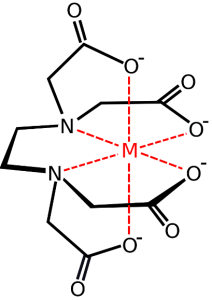
\includegraphics{Abb/EDTA.png}\\
  Abb.1: Ethylendiamintetraacetat (EDTA) als Chelatkomplexbildner um ein Metallkation \ce{M^{4+}}
\end{center}

In Tabelle 1 sind die verbrauchten Volumina an Maßlösung gegeben, die bis zum Umschlagspunkt in die Aliquoten titriert wurden.\\
Die Gesamtstoffmenge lässt sich analog zur Stoffmenge von \ce{Zn^{2+}} berechnen und sind in Tabelle 1 gegeben.
\begin{align*}
  n_{\mathrm{Ges}} &= \Delta V_{\text{Maßlösung}} \cdot c_{\text{Maßlösung}} \cdot 10\\
  &= 0.0049\,\mathrm{l} \cdot 0.09999\,\mathrm{\frac{mol}{l}} \dot 10\\
  &= 4.89951\,\mathrm{mmol}
\end{align*}

\newpage

\begin{center}
  Tab.1: Verbrauchte Volumina nach Aliquoten wobei bei Aliquot 3 und 4 nur die Stoffmenge von \ce{Zn^{2+}} bestimmt wurde.\\
\begin{tabular}{l l l l}
  \hline
  Aliquot & $\Delta V_{\text{Maßlösung}}$ [ml] & $n_{Ges}$ [mmol] & $n_{\ce{Zn^{2+}}}$ [mmol]\\
  \hline
  1 & 4.90 & 4.8995 & -\\
  2 & 4.90 & 4.8995 & -\\
  3 & 2.75 & - & 2.7497\\
  4 & 2.60 & & 2.59975 \\
  \hline
  Mittelwert & & 4.8995 & 2.6747\\
\hline
\end{tabular}
\end{center}

Die Stoffmenge von \ce{Mg^{2+}} wird durch folgende Gleichung berechnet, hierfür werden jeweils die Mittelwerte aus Tabelle 1 genommen.
\begin{align*}
  n(\ce{Mg^{2+}}) &= n_{\mathrm{Ges}} - n(\ce{Zn^{2+}})\\
  &= 4.8995\,\mathrm{mmol} - 2.6747\,\mathrm{mmol}\\
  &= 2.2248\,\mathrm{mmol}
\end{align*}

Somit wurde eine Gesamtstoffmenge $n_{\mathrm{Ges}} = 4.8995\,\mathrm{mmol}$ und die zwei Stoffmengen $n(\ce{Zn^{2+}}) = 2.6747\,\mathrm{mmol}$ und $n(\ce{Mg^{2+}}) = 2.2248\,\mathrm{mmol}$ experimentell bestimmt.

\section{Literatur}
[1] Skript zum Praktikum im Modul AC I: 19.07.2023
\end{document}
